\section{Eshelby Test}
\label{sec:example_eshelbytest}
The Eshelby test benchmark is designed to validate the different mechanical solver that come along with OpenPhase, namely the \nameref{sec:module_spectralelasticsolver} by Hu and Chen \citeopref{Hu2001}, the \nameref{sec:module_spectralelasticsolverBS} by Moulinec and Suquet \citeopref{Moulinec1998}, the \nameref{sec:module_spectralelasticsolverAL} by Michel et al.\ \citeopref{Michel2000} as well as the SpectralElasticSolverAS by Eyre and Milton (soon).\\
A spherical inclusion is placed inside an infiniteley expanded elastic matrix. The sphere has an eigenstrain of $\varepsilon^*_{11} = \varepsilon^*_{22} = \varepsilon^*_{33} = 0.01$, both matrix and sphere have the same isotropic, elastic stiffness parameters. For such a setup, Eshelby \citeopref{Eshelby1957} derived an analytical solution for stress and strain field, which can be used to validate the
\subsection{Modules and parameters}
The benchmark uses the three mandatory modules \nameref{sec:module_phasefield}, \nameref{sec:module_boundaryconditions} and \nameref{sec:module_settings}. The aforementioned elastic solvers (\nameref{sec:module_spectralelasticsolver}, \nameref{sec:module_spectralelasticsolverBS} and \nameref{sec:module_spectralelasticsolverAL}) can be chosen by changing the preprocessor flag. In order to perform the mechanical calculations it is necessary to load \nameref{sec:module_elasticproperties} as well one of the two homogenization modules \nameref{sec:module_elasticityreuss} or \nameref{sec:module_elasticitykhachaturyan}, respectively. Tables~\ref{tab:EshelbyTest_prInput} and \cref{tab:EshelbyTest_elInput} summarize the most important parameters for the Eshelby test example. Note that in the numerical setup no infinitely large domain can be chosen.
\begin{table}[ht]
\centering
\begin{tabular}{lll}
\toprule
Key & Value & Comment \\
\midrule
\$nSteps & 0 & Single step\\
\$Nx & 129 & \multirow{3}{8cm}{Note: In order to obtain appropriate results, a minimum resolution of 128 per dimension is suggested.}\\
\$Ny & 129 & \\
\$Nz & 129 & \\
\$Nphses & 2 & Two phases\\
\$IWidth & 0 & No diffuse interface\\
\bottomrule
\end{tabular}
\label{tab:EshelbyTest_prInput}
\caption{ProjectInput.opi for Eshelby test}
\end{table}
\begin{table}[ht]
\centering
\begin{tabular}{lcc}
\toprule
Key & Value 1 & Value 2 \\
\midrule
\$Phase 0\\
\$C11 & 280,000 &  0\\
\$C22 & 280,000 &  0\\
\$C33 & 280,000 &  0\\
\$C12 & 120,000 &  0\\
\$C13 & 120,000 &  0\\
\$C23 & 120,000 &  0\\
\$C44 & 80,000 &   0\\
\$C55 & 80,000 &  0\\
\$C66 & 80,000 &  0\\
\bottomrule
\end{tabular}
\caption{ElasticityInput.opi for Eshelby test}
\label{tab:EshelbyTest_elInput}
\end{table}
\subsection{Results}
Comparisons can be obtained against the analytical solution of Eshelby \citeopref{Eshelby1957}.
\begin{equation}
 \sigma_{ii}=\left\{
\begin{array}{cl}
-\sigma_0 & \textrm{inside the particle; } x_1 < r_p\\
 -\sigma_0\left(\frac{r_p}{x_1}\right)^3 & \textrm{for } i=1; x_1 > r_p\\
 \frac{1}{2}\sigma_0\left(\frac{r_p}{x_1}\right)^3 & \textrm{for }i \neq 1; x_1 > r_p
 \end{array}\right.
 \label{eq:EshelbyTest_AnalyticalSolution}
\end{equation}
where
\begin{equation}
\sigma_0 = \frac{2}{3}\left(C_{11}+2C_{12}\frac{1-2\nu}{1-\nu}\varepsilon^*\right)
\end{equation}

\begin{figure}
\centering
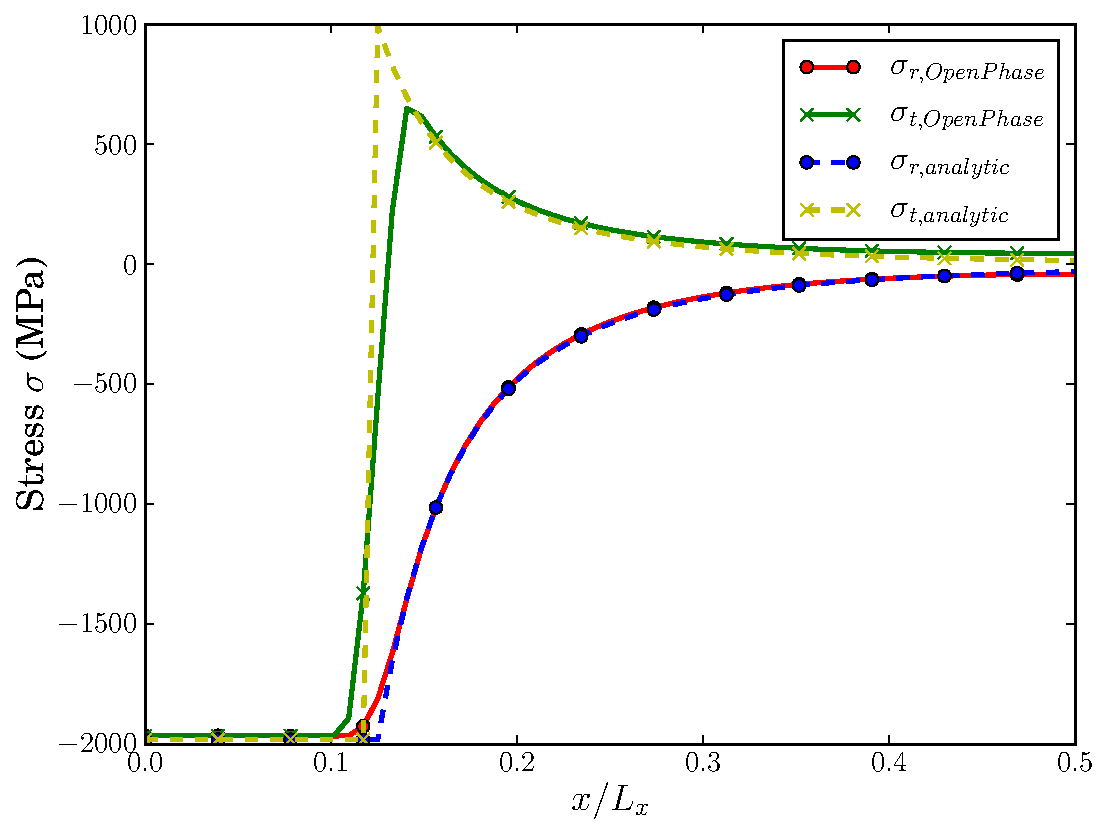
\includegraphics[width=0.8\textwidth]{examples/benchmark_eshelby.pdf}
\label{fig:example_eshelby}
\caption{Comparison of analytic Eshelby solution with results calculated by OpenPhase.}
\end{figure}
